\section{Iron --- Spin-orbit-coupled bands and Fermi-surface contours}
\label{sec17:IronSO}

\begin{itemize}
	\item Outline: {\it Plot the spin-orbit-coupled bands of ferromagnetic bcc Fe. Plot the Fermi-surface contours on a plane in the Brillouin zone.}
\end{itemize}

\begin{figure}[h!]
\centering
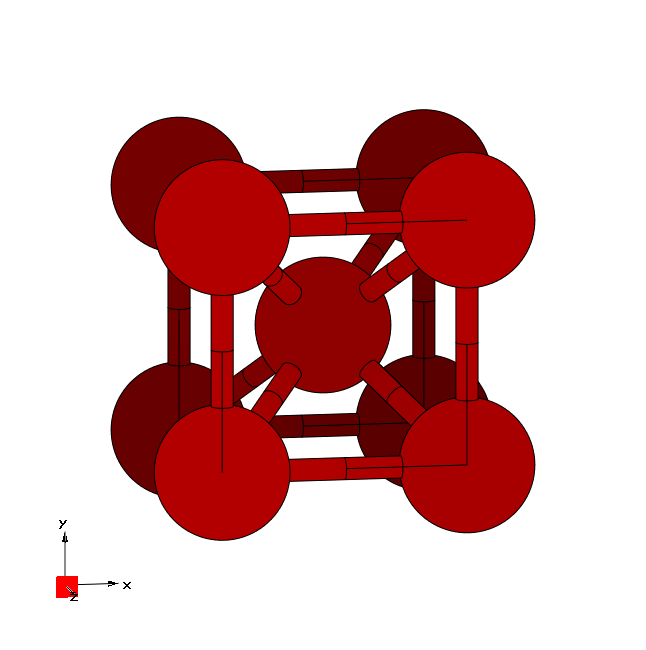
\includegraphics[width=0.25\columnwidth,trim={45pt 45pt 55pt 55pt},clip]{figure/example08/iron.png}
\caption{Unit cell of Iron crystal plotted with the \xcrysden{} program.}
\label{fig17.0}
\end{figure}


\begin{itemize}
	\item[1-6] {Compute the MLWFs and compute the energy eigenvalues and spin expectation values.} 

	The final state for all the 18 MLWFs is  
	\begin{tcolorbox}[sharp corners,boxrule=0.5pt]
	{\small
	\begin{verbatim}
	 Final State
  WF centre and spread    1  ( -0.709848,  0.000000,  0.000000 )     1.08973288
  WF centre and spread    2  ( -0.685480, -0.000000,  0.000000 )     1.10285536
  WF centre and spread    3  (  0.709848, -0.000000,  0.000000 )     1.08973288
  WF centre and spread    4  (  0.685480, -0.000000,  0.000000 )     1.10285536
  WF centre and spread    5  ( -0.000000, -0.709848,  0.000000 )     1.08973287
  WF centre and spread    6  (  0.000000, -0.685480,  0.000000 )     1.10285536
  WF centre and spread    7  (  0.000000,  0.709848,  0.000000 )     1.08973288
  WF centre and spread    8  (  0.000000,  0.685480,  0.000000 )     1.10285536
  WF centre and spread    9  (  0.000000, -0.000000, -0.709835 )     1.08977307
  WF centre and spread   10  (  0.000000, -0.000000, -0.685503 )     1.10302800
  WF centre and spread   11  ( -0.000000, -0.000000,  0.709835 )     1.08977304
  WF centre and spread   12  (  0.000000, -0.000000,  0.685503 )     1.10302800
  WF centre and spread   13  ( -0.000000, -0.000000, -0.000000 )     0.43232470
  WF centre and spread   14  ( -0.000000, -0.000000, -0.000000 )     0.41118748
  WF centre and spread   15  (  0.000000,  0.000000, -0.000000 )     0.43232470
  WF centre and spread   16  (  0.000000,  0.000000, -0.000000 )     0.41118748
  WF centre and spread   17  ( -0.000000,  0.000000,  0.000000 )     0.43232866
  WF centre and spread   18  ( -0.000000,  0.000000,  0.000000 )     0.41119649
  Sum of centres and spreads (  0.000000,  0.000000,  0.000000 )    15.68650457

         Spreads (Ang^2)       Omega I      =    11.898334117
        ================       Omega D      =     0.031570932
                               Omega OD     =     3.756599523
    Final Spread (Ang^2)       Omega Total  =    15.686504572
 ------------------------------------------------------------------------------
	\end{verbatim}
	}
	\end{tcolorbox}
	\item[] {\it To plot the bands using {\tt python}}
	{\tt
	\begin{quote}
	\$> python Fe-bands.py 
	\end{quote}
	}
	The interpolated band structure of Fe with spin-orbit interaction using the module {\tt kpath} is shown in \Fig{fig17.1}. The color scheme is used to show the expectation value of the spin operator $\hat{S}_z$ in units of $\hbar/2$.
	\begin{figure}[h!]
	\centering
	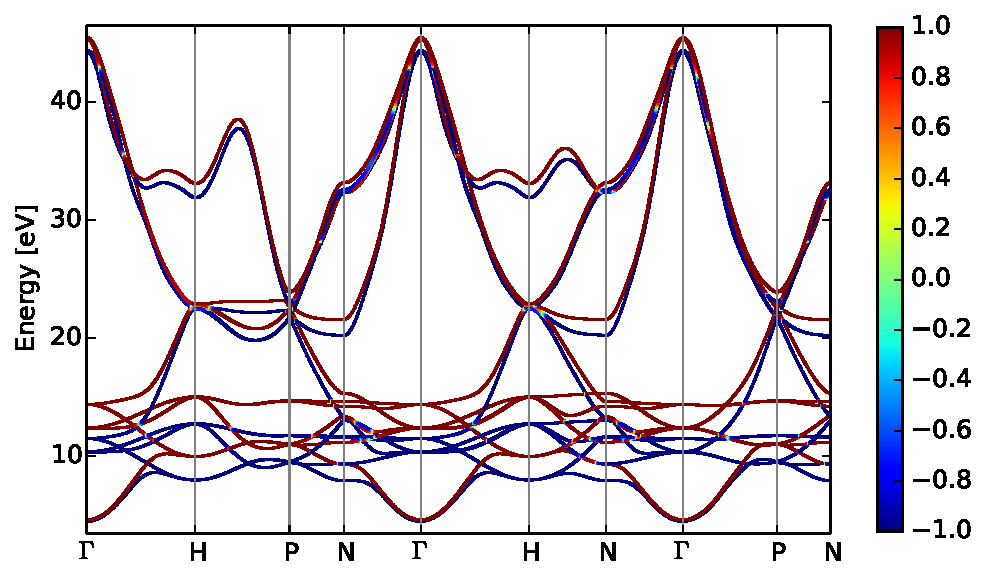
\includegraphics[width=0.6\columnwidth]{figure/example17/Fe_bandstructure.pdf}
	\caption{\Wannier{} interpolated bands of Fe computed from a DFT calculation with spin-orbit interaction. Colour-scheme shows the expectation value $\braket{\hat{S}_z}$ in units of $\hbar/2$.}\label{fig17.1}
	\end{figure}
	\item[]{\it Next we plot the Fermi-surface contours on the (010) plane $k_y = 0$, using the {\tt kslice} module.}

	\begin{figure}
	\centering
	\subfloat[spin-orbit {\tt kslice}]{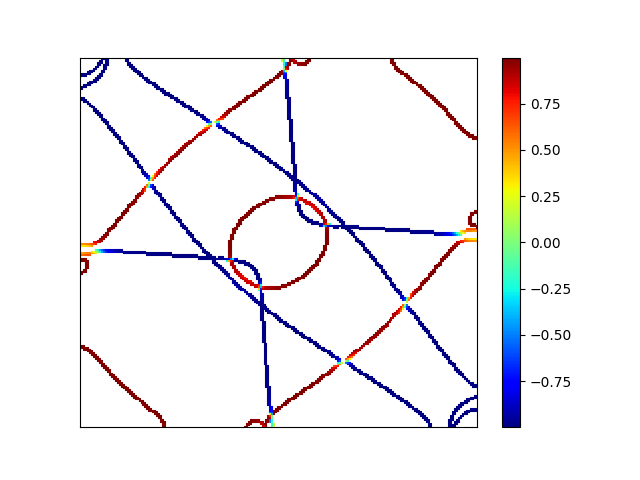
\includegraphics[width=0.45\columnwidth]{figure/example17/Fe-kslice-fermi_lines_lowres.png}}
	\centering
	\subfloat[no spin-orbit]{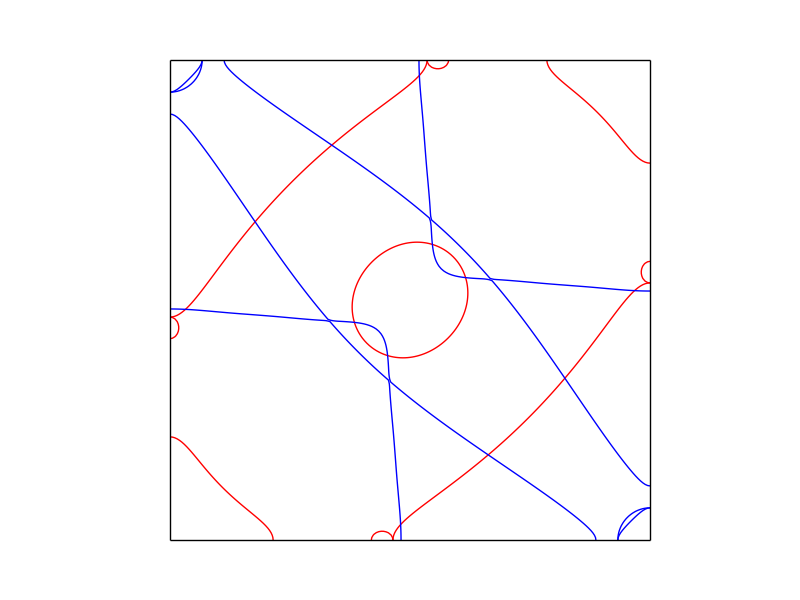
\includegraphics[width=0.45\columnwidth]{figure/example17/Fe_Fermi_surface.png}}	
	\caption{}\label{fig17.2}
	\end{figure}

	\subsection*{Further ideas}
	\begin{itemize}
		\item {\it Redraw the Fermi surface contours on the (010) plane starting from a calculation without spin-orbit coupling (SOC), by adding to the input files iron\_\{up,down\}.win in Example 8.}

		The Fermi surface contours on the (010) plane without SOC are shown in \Fig{fig17.4}-(a).
		\item {\it For a spinor calculation we can still spin-decompose the DOS.}
		\begin{figure}[h!]
		\centering
		\subfloat[spin-decomposed]{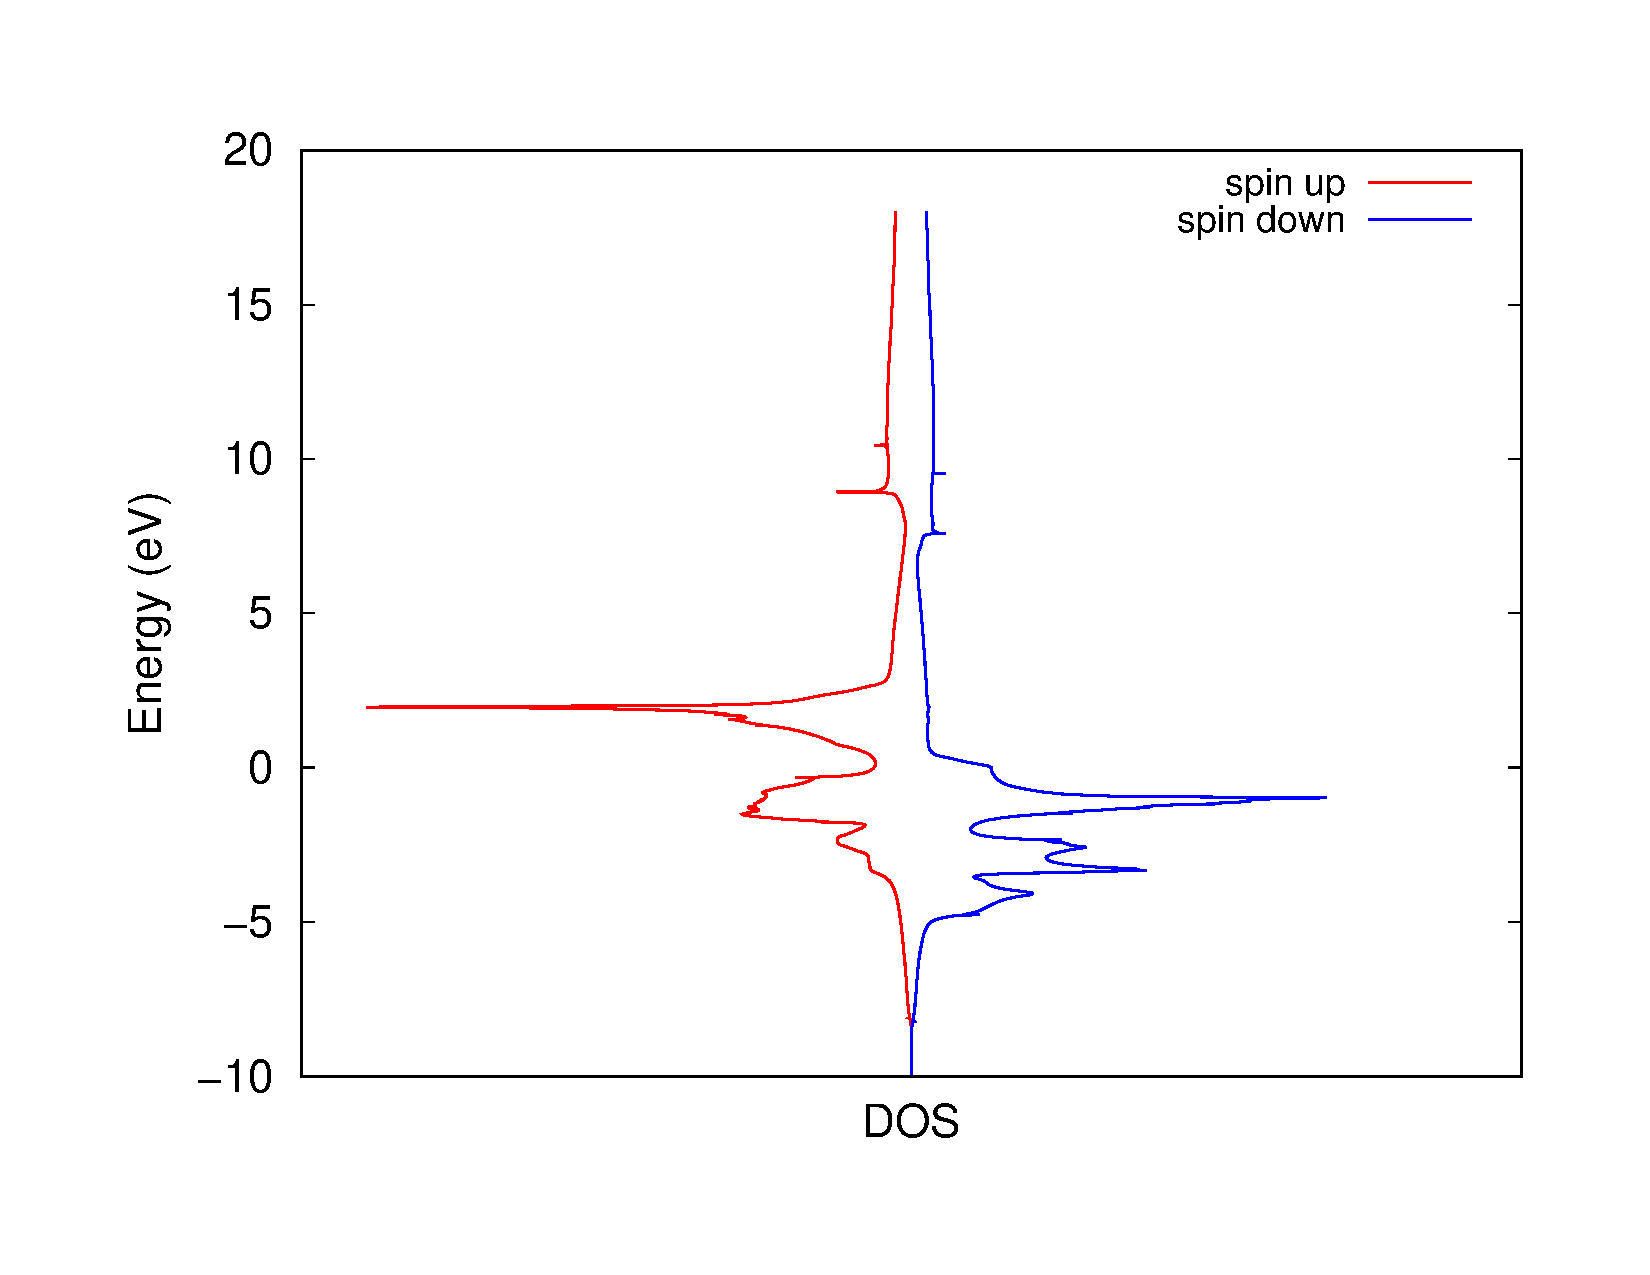
\includegraphics[width=0.45\columnwidth]{figure/example17/DOS_Fe_bcc.pdf}}
		\centering
		\subfloat[projected]{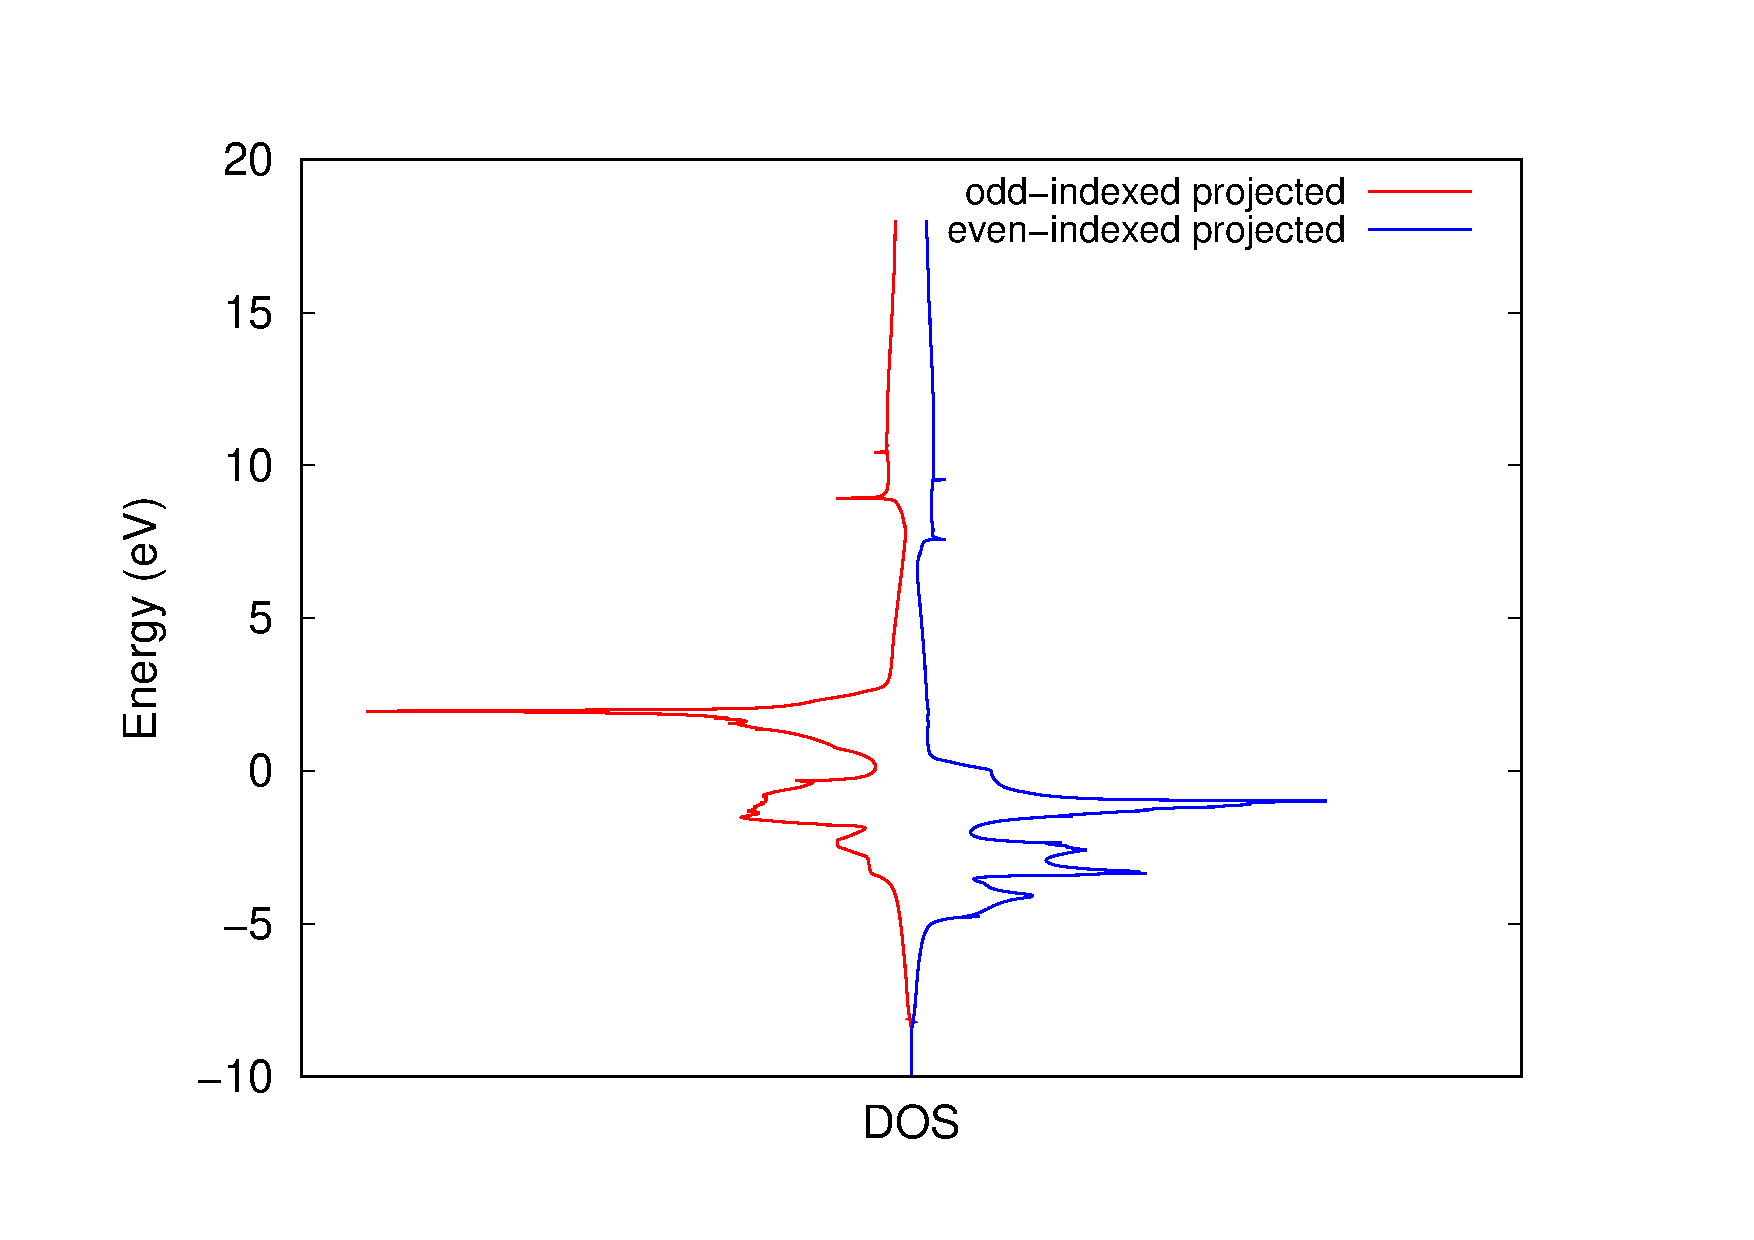
\includegraphics[width=0.45\columnwidth]{figure/example17/DOS_Fe_bcc_projected.pdf}}
		\caption{Spin-decomposed DOS (panel a) with spin-up (red) and spin-down (blue) components. Projected DOS on odd-indexed MLWFs (red) and even-indexed (blue).}\label{fig17.4}
		\end{figure}
	\end{itemize}
\end{itemize}
